\chapter{CompensadorAnalogico} \chapterlabel{Informe/6-CompensadorAnalogico} \label{cap:Compensador Analogico}

\section{Compensador Analogico}

\noindent Se plantea una compensación como la que se muestra en la figura \ref{fig:diag-en-bloques-comp}. Está compuesta por un lazo de control interno con un controlador por adelanto de fase para lograr estabilizar el sistema, y un lazo de control externo con un integrador para eliminar el error en régimen permanente.

\begin{figure}[H]
	\centering
	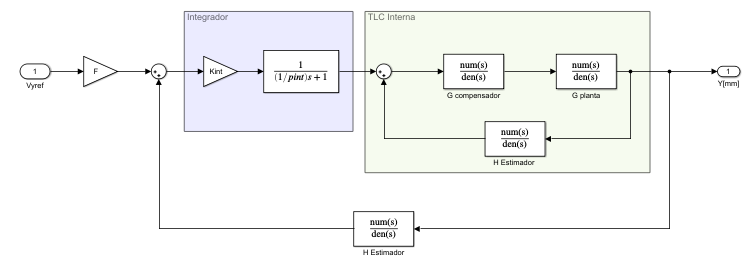
\includegraphics[scale=1]{Diagrama-en-bloques-comp.png}
	\caption{Diagrama del sistema completo.}
	\label{fig:diag-en-bloques-comp}
\end{figure}

\subsection{Diseño de compensador por adelanto de fase}

\noindent A partir de las transferencias de la planta, el controlador de corriente y el estimador de posición, se realizó el diseño de un compensador analógico por el método de adelanto de fase. Se llegó a la siguiente transferencia:


\begin{equation} 
	G_c(s) = 10*[20.346 * \frac{(s+44.3)}{(s+902.1)}]^2
\end{equation}

\noindent A continuación se diseña un circuito analógico correspondiente a este compensador.

\subsection{Diseño circuital}

\begin{figure}[H]
	\centering
	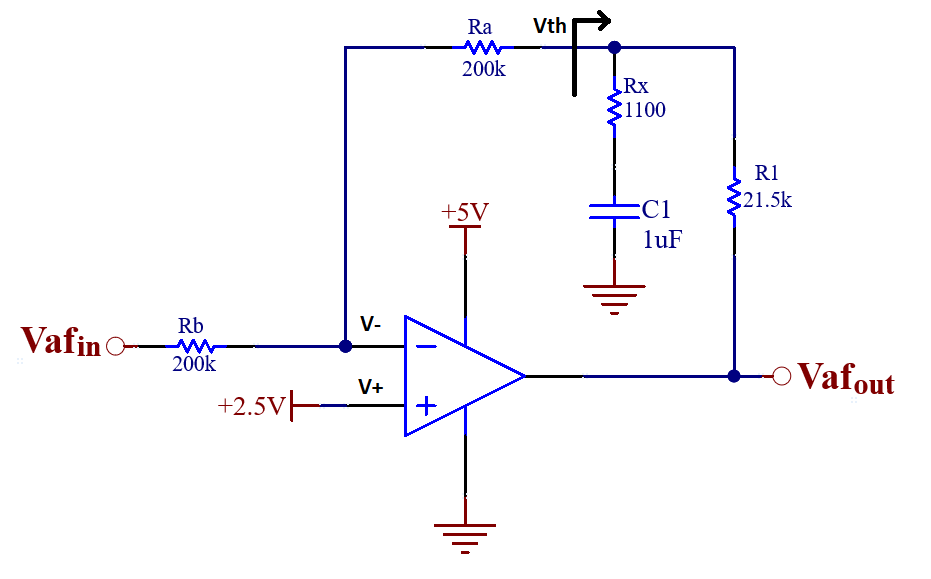
\includegraphics[scale=0.6]{Red-adelanto-fase.png}
	\caption{Diseño circuital de una red de adelanto de fase.}
	\label{fig:red-adelanto-fase}
\end{figure}


\noindent Para cada etapa del compensador por adelanto, se utilizará la topología mostrada en la figura \ref{fig:red-adelanto-fase}. Consiste en  un polo y cero con ganancia unitaria (si Ra = Rb). Luego se agrega la ganancia como una etapa separada.

\noindent La transferencia de lazo cerrado de esta etapa es:

\begin{equation} 
	\frac{V_{out}}{V_{in}}= - \frac{R_a}{R_b}*\frac{1+sC(R_x+R1)}{1+sCR_x}
\end{equation}

